\documentclass[tikz,border=10pt]{standalone}

\usepackage{tikz}
\usetikzlibrary{arrows.meta, positioning}

\begin{document}

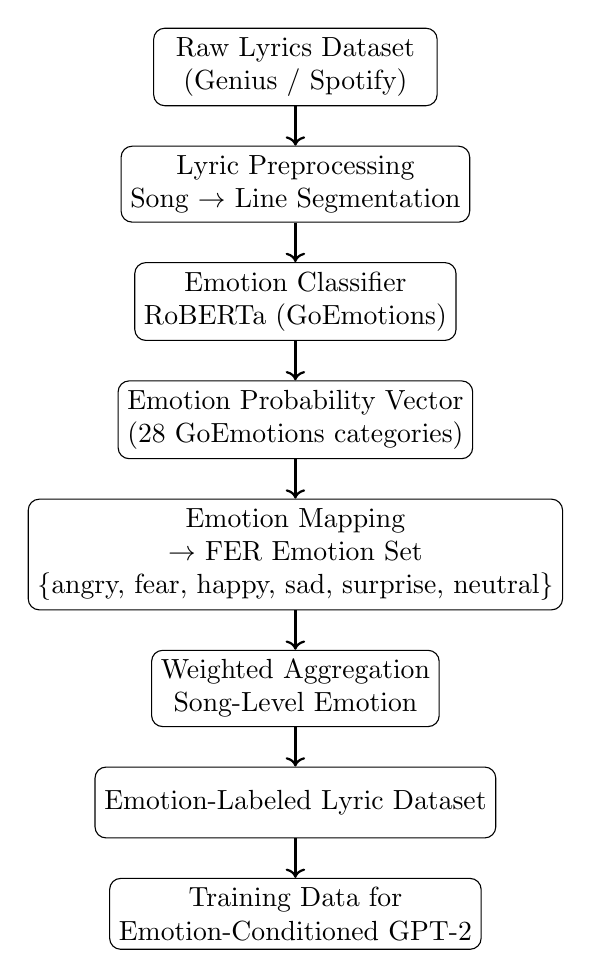
\begin{tikzpicture}[
node distance=0.5cm,
box/.style={draw, rectangle, rounded corners, align=center, minimum width=3.6cm, minimum height=0.9cm},
arrow/.style={->, thick}
]

\node[box] (dataset)
{Raw Lyrics Dataset\\
(Genius / Spotify)};

\node[box, below=of dataset] (segment)
{Lyric Preprocessing\\
Song $\rightarrow$ Line Segmentation};

\node[box, below=of segment] (classifier)
{Emotion Classifier\\
RoBERTa (GoEmotions)};

\node[box, below=of classifier] (prob)
{Emotion Probability Vector\\
(28 GoEmotions categories)};

\node[box, below=of prob] (mapping)
{Emotion Mapping\\
$\rightarrow$ FER Emotion Set\\
$\{$angry, fear, happy, sad, surprise, neutral$\}$};

\node[box, below=of mapping] (aggregate)
{Weighted Aggregation\\
Song-Level Emotion};

\node[box, below=of aggregate] (dataset2)
{Emotion-Labeled Lyric Dataset};

\node[box, below=of dataset2] (training)
{Training Data for\\
Emotion-Conditioned GPT-2};

\draw[arrow] (dataset) -- (segment);
\draw[arrow] (segment) -- (classifier);
\draw[arrow] (classifier) -- (prob);
\draw[arrow] (prob) -- (mapping);
\draw[arrow] (mapping) -- (aggregate);
\draw[arrow] (aggregate) -- (dataset2);
\draw[arrow] (dataset2) -- (training);

\end{tikzpicture}

\end{document}
